% Format adapted from archive/legacy/docs/geccoPaper/main.tex; historical text untouched.
\ifdefined\namedversion
\documentclass[sigconf,dvipsnames]{acmart}
\else
\documentclass[sigconf,dvipsnames,anonymous,review]{acmart}
\fi
\setcopyright{none}
\settopmatter{printacmref=false}
\acmDOI{}
\acmISBN{}
\acmConference[ManiGuard pilot]{ManiGuard pilot in GECCO format}{18 October 2026}{}
\usepackage{xurl}
\setlength{\emergencystretch}{3em}
\graphicspath{{../../figures/ManiGuard/phase3-part1/}}
\begin{document}
\title{An Evolutionary Safety Dial for Frozen Manipulation Policies: A Physically Audited Pilot}
\subtitle{Frozen-protocol research report, 18 October 2026}
\author{Sachin Mohan}
\affiliation{\institution{University of the Witwatersrand}\city{Johannesburg}\country{South Africa}}
\email{2699183@students.wits.ac.za}
\renewcommand{\shortauthors}{Mohan}
\begin{abstract}
Can evolutionary search discover a compact execution controller that improves safe
completion around a frozen manipulation policy? We implement a four-parameter
controller and external intervention-strength dial in ManiGuard Clutter. A frozen
single-seed protocol allocates 24 simulator episodes to search and 24 fresh episodes
to comparing one frozen finalist at dial strengths zero, one-half and one. The
finalist safely completes both final training episodes. This gain does not persist:
identity achieves 5/8 safe completions with no observed violating episode; half
strength achieves 3/8 with two violations; full strength achieves 4/8 with two
violations. Full strength completes more tasks overall, but two completions are
unsafe. Query cost falls, without a safe-completion improvement. We preserve all
52 attempts including engineering, complete action/monitor traces, source and
checkpoint hashes, three-setting videos, and continuous allocated-time accounting.
This is an adverse descriptive result on two exposed scenes, not evidence that
evolution outperforms other search methods or that the dial calibrates physical risk.
\end{abstract}
\begin{CCSXML}
<ccs2012><concept><concept_id>10010147</concept_id>
<concept_desc>Computing methodologies</concept_desc>
<concept_significance>500</concept_significance></concept></ccs2012>
\end{CCSXML}
\ccsdesc[500]{Computing methodologies}
\keywords{evolutionary search, execution adaptation, manipulation, safety, frozen policies}
\maketitle

\section{Question and scope}
Task completion can conceal a manipulation policy's physical specification
violations. ManiGuard separates task success from safety using runtime monitors
over physics-grounded predicates~\cite{maniguard}. We test whether a small execution
controller can improve safe completion around a frozen Clutter policy, and whether
an external dial exposes a useful measured trade-off. All physical outcomes here
are measured in simulation. The monitor labels actions' consequences; it does not
filter commands.

This pilot implements the Part 1 plan at planning commit \texttt{8df7ac9}. The
machine-readable protocol was frozen before search. It contains the controller
domain, information restrictions, source hashes, scene partitions, schedules,
selection rules and absolute deadlines. The work establishes an executable and
auditable experiment. It provides no optimizer-superiority or safety-guarantee claim.

\section{Controller and frozen protocol}
The genome has four categorical coordinates: free-motion joint-target cap
$\{\varnothing,.12,.08,.04\}$ rad, grasp cap
$\{\varnothing,.08,.04,.02\}$ rad, smoothing $\{1,.75,.5\}$, and query horizon
$\{4,8,16\}$. This defines 144 points. The neutral genome disables caps and uses
smoothing one and horizon eight.

For proposed arm targets $p$, measured joints $q$ and smoothing $\alpha$, define
$r=q$ on the first action and the previous actual environment input thereafter.
The anchor computes
\begin{equation}
 z=r+\alpha(p-r),\qquad
 a=q+\operatorname{clip}(z-q,-c,c),
\end{equation}
with $a=z$ when the applicable cap is disabled. The fixed causal finger heuristic
selects the grasp cap: absolute finger positions are in $[.003,.035]$, their
maximum change is below $.002$, and the proposal closes the gripper. It does not
identify the held object.

The episode-constant external dial $d$ applies $p+d(a-p)$ to the arm and uses
\begin{equation}
 h(d)=\left\lfloor8+d(h_\theta-8)+.5\right\rfloor.
\end{equation}
Zero bypasses arithmetic exactly; one returns the anchor directly. Native gripper
binarization, downstream clipping and termination remain intact. History updates
from the final clipped environment input, before low-level actuator processing.
The controller uses only proposals, measured arm/finger positions and that causal
history. Object states, goal labels and monitor predicates are excluded. Caps
bound target displacement rather than force or collision probability.

Search runs only at $d=1$, using PCG64 seed 20261018. Population zero contains
identity and three distinct uniform random points. Each of three populations has
four slots, evaluated on two training assignments. The next population copies
the best point for fresh physical re-evaluation and creates three mutated children
from the best two parents. The declared categorical mutation kernel rejects
unchanged children and within-population duplicates; stable birth order resolves
ties, with the copied elite first. Fitness is
\begin{equation}
 \overline U=\operatorname{mean}\bigl[\mathbf1(S_{\rm req})-2\mathbf1(V)\bigr],
\end{equation}
where $V$ is raw \texttt{ltl\_violated}, $C_{\rm req}$ combines native success with
the pinned Clutter checklist, and $S_{\rm req}=C_{\rm req}\land\neg V$.
Infrastructure failures have no fitness. Only the final evaluated population can
supply the finalist.

Engineering uses \texttt{task\_0040/base}; search uses tasks 0034 and 0002; comparison
uses tasks 0029 and 0032. Whole-task partitions are preserved and test scenes remain
untouched. Training base seeds are $1000+10g+i$; comparison uses $2000+10j+r$ with
four repetitions per scene. The native evaluator derives sampling seeds as CRC32
of the base seed and scene, masked to 31 bits. The server resets a stream for each
episode ID. Independent schedule seed 20261019 seals adjacent three-dial blocks,
cycling all six permutations before repetition. Scenes are conservatively treated
as exposed; the comparison tests fresh repetitions.

\begin{figure*}[t]
\centering
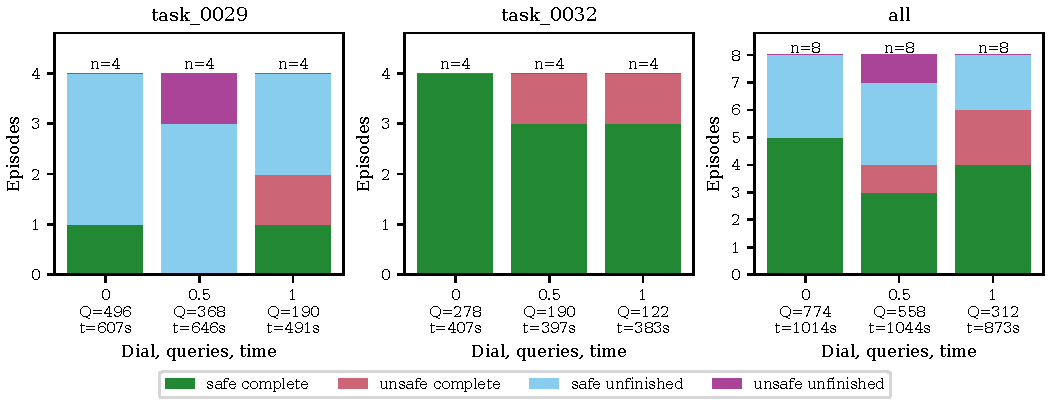
\includegraphics[width=\textwidth]{paper-outcomes.pdf}
\caption{Every fresh outcome, per scene and pooled. Each scene has four episodes per
setting; pooled denominators are eight. $Q$ is policy queries and $t$ is summed outer
episode-process time. Unsafe completion remains separate from safe completion.}
\Description{Three stacked bar charts show identity with five pooled safe completions
and zero violations, midpoint with three safe completions and two violations, and
full strength with four safe completions and two violations.}
\label{fig:outcomes}
\end{figure*}

\section{Search and fresh comparison}
Population-zero timing selected the full 48-episode allocation before selection
inspected scores. The shared eight episodes count once. The planning duration was
$\max(417\text{ s},1.25\times\text{slowest})=417$ s; the remaining estimate was
16,980 s against 21,149.97 s available. The predefined 28-episode fallback was unused.
All full jobs retain the native 1,100-action horizon and native early success.

\begin{table}[t]
\caption{Every population's mean candidate utilities, in birth order. The elite is
physically re-evaluated rather than retaining historical fitness.}
\label{tab:search}
\begin{tabular}{clcc}
\toprule
Population & Utilities & Safe complete & Violating \\
\midrule
0 & .5, 1, .5, 1 & 6/8 & 0/8 \\
1 & 1, 1, 0, .5 & 5/8 & 0/8 \\
2 & .5, 1, .5, $-.5$ & 5/8 & 1/8 \\
\bottomrule
\end{tabular}
\end{table}

The selected genome is $[3,3,0,2]$: free cap .04 rad, grasp cap .02 rad, smoothing
one, horizon sixteen. It is a new offspring of population one's second eligible
parent. It safely completes both final training episodes. The copied elite scores
only .5 in its last re-evaluation (Table~\ref{tab:search}, Figure~\ref{fig:lineage}).
One discarded search candidate completes unsafely; its outcome and costs remain.
The finalist's file hash is sealed before comparison, and all three settings use it.

\begin{figure}[t]
\centering
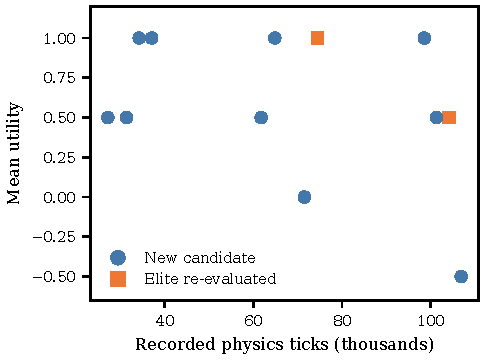
\includegraphics[width=\linewidth]{paper-lineage.pdf}
\caption{All twelve candidate measurements versus cumulative recorded physics ticks,
including engineering and the failed check. Squares distinguish re-evaluated elites.
These mixed-candidate measurements are not a single policy's estimated rate.}
\Description{Candidate mean utilities range from minus one half to one. The retained
elite falls from one to one half on its final fresh seed pair.}
\label{fig:lineage}
\end{figure}

Fresh safe completion is 5/8 at identity, 3/8 at midpoint and 4/8 at full strength
(Figure~\ref{fig:outcomes}). Full minus identity is $-1/8$, or $-12.5$ percentage
points, with two additional violating episodes. Full strength achieves six total
requested completions, but two are unsafe. Benchmark success and requested
completion agree on all 24 comparison episodes, with separate labels preserved.
No setting is selected or tuned against these outcomes.

On task 0029, safe completions are 1/4, 0/4 and 1/4. On task 0032, they are 4/4,
3/4 and 3/4. Each adapted setting records one violation on each scene. The first
failing predicate is \texttt{container\_upright=false} on task 0029 and
\texttt{obstacles\_upright=false} on task 0032. Both full-strength violating episodes
later reach the goal. The three-point response supports no calibrated or monotonic
physical-risk interpretation (Figure~\ref{fig:dial}).

\begin{figure}[t]
\centering
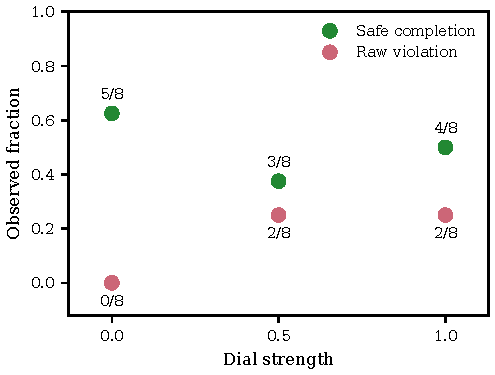
\includegraphics[width=\linewidth]{paper-dial-response.pdf}
\caption{Measured safe-completion and violation fractions with explicit denominators.
Points are descriptive; no continuous risk curve is fitted.}
\Description{Safe-completion fractions are five eighths, three eighths and four
eighths; raw violation fractions are zero, two eighths and two eighths.}
\label{fig:dial}
\end{figure}

\begin{table}[t]
\caption{Fresh interaction and process costs. Changed commands compare exact
numerical inputs; cap activation is reported separately in the audit.}
\label{tab:cost}
\begin{tabular}{crrrr}
\toprule
Dial & Actions & Queries & Process (s) & Changed \\
\midrule
0 & 6,160 & 774 & 1,014.0 & 0.00\% \\
.5 & 6,656 & 558 & 1,043.6 & 4.51\% \\
1 & 4,928 & 312 & 873.5 & 8.36\% \\
\bottomrule
\end{tabular}
\end{table}

Query latency totals are 76.8, 55.2 and 31.3 s respectively. Lower query cost at full
strength accompanies worse measured safety and safe completion; changing commands
and query horizon together prevents a mechanism-specific causal claim.
Contact/grasp episode counts, each out of eight, are $(5,5)$, $(5,4)$ and $(7,6)$.
The grasp heuristic activates on 955 midpoint and 1,325 full-strength actions; anchor
caps activate on 235 and 350. Identity's diagnostic anchor counters do not change
commands. Non-engagement in several unfinished episodes limits interpretation of
zero violations alone.

\begin{figure}[t]
\centering
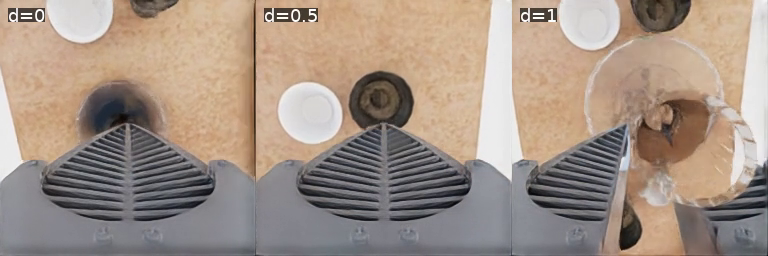
\includegraphics[width=\linewidth]{frames/task_0029-base-seed2000-wrist-t18s.png}\par
\smallskip
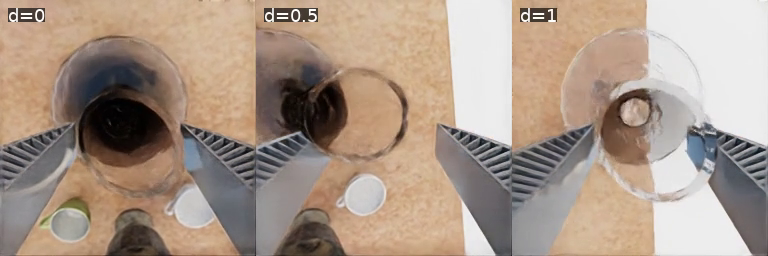
\includegraphics[width=\linewidth]{frames/task_0029-base-seed2002-wrist-t18s.png}\par
\smallskip
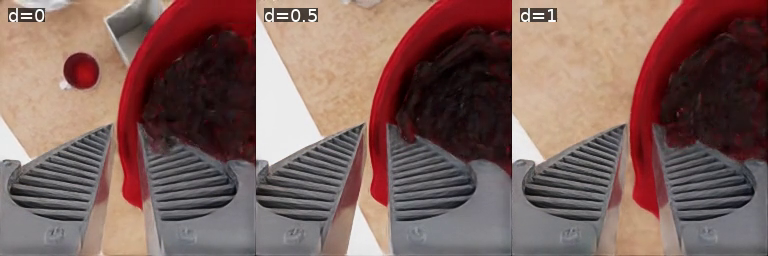
\includegraphics[width=\linewidth]{frames/task_0032-base-seed2013-wrist-t18s.png}
\caption{Actual wrist-video frames at 18 s; columns are dial 0, .5 and 1. Top:
seed 2000, where full strength later safely completes while the other settings time
out. Middle: seed 2002, where midpoint and full strength lose container uprightness;
full strength later completes unsafely. Bottom: seed 2013, where full strength loses
an obstacle's uprightness before its unsafe completion. These illustrations were
selected after outcomes. All sixteen fixed-time camera strips and all sixteen
complete three-setting videos are saved, covering every block. No physics is replayed.}
\Description{Three matched wrist-image strips show the same scene and nominal time
under the three dial settings, including the initially promising and adverse cases.}
\label{fig:frames}
\end{figure}

\section{Engineering, accounting and provenance}
CPU verification passes 33 Part 1 tests and 109 regression tests, with four skips.
Checks cover identity, causal clipped-action history, caps, finger switching,
interpolation, query schedules, seeded evolution, evidence corruption and owned
process-group cleanup. Three successful engineering checks use 32 actions each and
4/6/8 queries for an engineering horizon-four anchor. Chunks support horizon sixteen.
One earlier check fails after one completed query and zero policy actions because
strict JSON rejects infinite native action bounds. Logging is fixed before search,
without changing clipping. A naming bug produces nested engineering paths; these
are preserved and the coordinator is repaired before search. All 48 full episodes
pass physical trace replay and provenance audits.

\begin{table}[t]
\caption{Complete attempt accounting. Physics covers post-application callbacks;
pre-subscription advances are unknown for all 52 attempts.}
\label{tab:ledger}
\begin{tabular}{lrrrr}
\toprule
Work & Attempts & Actions & Queries & Physics ticks \\
\midrule
Engineering & 4 & 96 & 19 & 920 \\
Search & 24 & 17,318 & 1,738 & 105,972 \\
Comparison & 24 & 17,744 & 1,644 & 108,528 \\
Total & 52 & 35,158 & 3,401 & 215,420 \\
\bottomrule
\end{tabular}
\end{table}

All 3,401 queries complete; the failed check is a logging failure. There are 35,678
environment-step attempts and returns, 1,795.17 recorded simulated seconds, 360.03 s
of query latency and 5,982.17 s of outer episode-process time. Counts include all
initialization, discarded candidates and copied elites. Pre-subscription physics
is unknown, not zero; failed-attempt counters remain lower bounds. Overlapping
server durations do not add allocated GPU-hours.

The user-confirmed replacement is Vast instance 56582094 with one RTX 4090 and driver
575.57.08, verified through the kernel, \texttt{nvidia-smi} and provider. The originally
requested 56578764 identity is retained as provenance. No host driver is changed.
Five-second memory samples reach 17,714 MiB (17.3 GiB), without bounding unobserved
peaks. CPU/memory quotas are 30.6 cores and approximately 299 GiB.

Separate uv-managed Python 3.10 simulation and Python 3.11 policy environments use the
pinned ManiGuard, BEHAVIOR and openpi stack~\cite{openpi}. The checked legacy renderer
supplies $256\times256$ RGB overview/wrist inputs with action/render/physics rates
20/20/120 Hz, raw joint control and assisted grasping. The root environment and
UNISafe installers are not used. Clutter checkpoint revision
\texttt{f572e33bdb49} (full revision in the controller export), step 7100, keeps native inference
settings. Controller exports retain all eighteen checkpoint-file hashes and code pins.

The original allocation clock starts at 16:00:37 UTC, including setup, implementation,
failed and idle work before and after replacement. An independent supervised guard
preserves the 23:00:37 UTC physical target and 00:00:37 UTC next-day hard end across
restarts. The policy stops at 18:25:29 UTC; process/GPU checks confirm complete exit
by 18:25:57 UTC, at 2.422 allocated GPU-hours. Subsequent paper preparation, backup
and idle rental continue to count. The public audit records the later accounting
cutoff and rental-stop scope.

The evidence contains 104 native video files, including the failed check, and sixteen
matched composites covering both cameras in all eight comparison blocks. CPU
composition preserves frame order and marks ended episodes with black frames.
A 52-row public ledger, lineage, fixed-time picture gallery, frozen protocol and
controller, and all figure data accompany this note. Credential-scanned raw evidence
is preserved in the approved private dataset, with asset bundles, checkpoints and
keys excluded. The \href{https://huggingface.co/datasets/Sachioster/safety-dial-phase3-part1-20261018/tree/17dbdcb7e29a71c763f6441ac4aa8d0c7fcf6647/matched-videos}{matched-video gallery}
requires the owner's access. Git contains derived reporting artifacts rather than
raw run directories.

\section{Limitations and conclusion}
The training lead disappears in the fresh check. The controller increases observed
violations and does not improve safe completion. It is a working interface with an
adverse pilot result. Matching seeds does not equate observations: all sixteen initial
state comparisons are numerically identical, but every camera-image comparison
differs. Two exposed scenes, eight repetitions per setting and one optimizer seed
support only a descriptive conclusion. Identity's zero violations would give the
approximate 95\% upper bound $3/8=37.5\%$ even under independent homogeneous sampling;
repeated scenes further limit interpretation.

A new allocation should isolate query scheduling from caps and compare strong fixed
settings and matched random search before increasing evolutionary search. Ordinary
policy learning remains necessary for the broader research claim. This allocation
contains none of those comparisons and no outcome-dependent extra episodes.

\begin{acks}
AI coding assistance was used for implementation, analysis code, prose and typesetting.
Experimental outcomes derive from the recorded simulator/monitor traces, and every
experimental picture is extracted from native video. The paper adapts the repository's
existing GECCO template without changing its archived experiment or results.
\end{acks}
\bibliographystyle{ACM-Reference-Format}
\bibliography{references}
\end{document}
